\subsubsection{Quản lý tổ chức}
\begin{figure}[H]
    \centering
    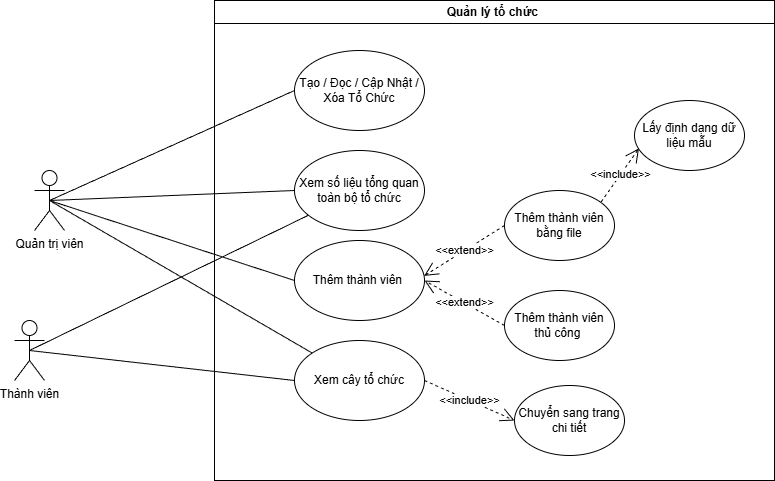
\includegraphics[width=1.0\linewidth]{Images/use-case-diagram/UC04_organizations_usecase.drawio.png}
    \vspace{0.3em}
    \caption{UC04 -  Quản lý tổ chức}
    \label{fig:uc01-usecase}
\end{figure}
\renewcommand{\arraystretch}{1.3}
\begin{longtable}{|m{0.25\textwidth}|m{0.75\textwidth}|}
\hline

\textbf{Use-case Name} & \textbf{UC04. Quản lý tổ chức} \\ \hline
\endfirsthead

\hline
\textbf{Use-case Name (tiếp)} & \textbf{UC04. Quản lý tổ chức} \\ \hline
\endhead

% ===== Nội dung bảng =====
\textbf{Actors} 
& \begin{itemize}[label=--]
    \item Quản trị viên (Admin)
    \item Thành viên (Member) 
\end{itemize} \\ 
\hline

\textbf{Description} 
& Cho phép người dùng xem cấu trúc cây tổ chức và số liệu thống kê tổng quan. 
Đối với Quản trị viên, hệ thống cung cấp các chức năng quản lý nâng cao như: Tạo/Sửa/Xóa tổ chức và Thêm thành viên (hỗ trợ thêm thủ công hoặc nhập từ file). \\ 
\hline

\textbf{Trigger} 
& Người dùng truy cập vào trang "Quản lý tổ chức" từ thanh điều hướng chính. \\ 
\hline

\textbf{Pre-Conditions} 
&
\begin{itemize}[label=--]
    \item Người dùng đã đăng nhập vào hệ thống.
    \item Dữ liệu về tổ chức và thành viên đã tồn tại trong cơ sở dữ liệu.
\end{itemize}
\\ 
\hline

\textbf{Post-Conditions} 
&
\begin{itemize}[label=--]
    \item Hiển thị chính xác cấu trúc cây tổ chức và số liệu thống kê.
    \item Các thay đổi về cấu trúc tổ chức hoặc thành viên mới (nếu có) được cập nhật vào hệ thống.
\end{itemize}
\\ 
\hline

\textbf{Normal Flow} 
&
\begin{enumerate}
    \item Người dùng yêu cầu xem danh sách tổ chức.
    \item Hệ thống tải và hiển thị dữ liệu dưới dạng cây phân cấp (Tree View) kèm theo các số liệu thống kê tổng quan.
    \item Người dùng tương tác mở rộng/thu gọn các nhánh của cây tổ chức.
    \item Người dùng chọn một đơn vị tổ chức cụ thể.
    \item \textbf{(Include)} Hệ thống thực hiện quy trình \textit{"Chuyển sang trang chi tiết"} để hiển thị thông tin đầy đủ của tổ chức đó.
\end{enumerate}
\\ 
\hline

\textbf{Alternative Flow} 
& Tại bước 3 (Chức năng dành cho Quản trị viên - Thêm thành viên):
\begin{itemize}
    \item \textbf{3a.} Quản trị viên chọn chức năng "Thêm thành viên" vào tổ chức.
    \item \textbf{3b.} Hệ thống cung cấp 2 tùy chọn:
    \begin{itemize}
        \item \textbf{(Extend 1) Thêm thủ công:} Quản trị viên nhập thông tin từng thành viên vào form.
        \item \textbf{(Extend 2) Thêm bằng file:} Quản trị viên chọn tải lên danh sách từ file Excel/CSV.
        \item \textit{Trong trường hợp chọn Thêm bằng file:} \textbf{(Include)} Hệ thống cung cấp chức năng \textit{"Lấy định dạng dữ liệu mẫu"} để người dùng tải về template trước khi nhập liệu.
    \end{itemize}
\end{itemize}
\\ 
& Tại bước 3 (Chức năng quản lý cấu trúc):
\begin{itemize}
    \item \textbf{3c.} Quản trị viên thực hiện các thao tác CRUD: Tạo mới, Cập nhật thông tin hoặc Xóa một tổ chức khỏi cây.
\end{itemize}
\\
\hline

\textbf{Exception} 
& 
\begin{itemize}
    \item \textbf{Lỗi định dạng file:} Khi thực hiện "Thêm thành viên bằng file", nếu file không đúng mẫu, hệ thống báo lỗi và yêu cầu tải lại template chuẩn.
    \item \textbf{Lỗi dữ liệu:} Khi "Tạo/Sửa tổ chức", nếu tên tổ chức bị trùng hoặc thiếu thông tin bắt buộc, hệ thống hiển thị thông báo lỗi tương ứng.
\end{itemize}
\\
\hline
\caption{Bảng mô tả Use Case UC04 - Quản lý tổ chức}
\end{longtable}